% =====================================================================
%  Rapport de Projet de Fin d'Études - ENSIM
%  Ahmed BOURAZZA - VINCI Energies Systèmes d'Information (VESI)
%  Compilation : pdfLaTeX  (Overleaf : Menu > Compiler > pdfLaTeX)
%  Bibliographie : Biber
% =====================================================================
\documentclass[12pt,a4paper,twoside]{report}% --- Préambule (packages, police Times, marges, styles) ---
% =====================================================================
%  PRÉAMBULE
%  Contraintes ENSIM : Times New Roman 12, interligne simple,
%  marges 2 cm, pagination, labels figures/tableaux >= 9 pt.
% =====================================================================

% ---- Encodage et langue ----
\usepackage[utf8]{inputenc}
\usepackage[T1]{fontenc}
\usepackage[french]{babel}
\usepackage{csquotes}

% ---- Police : équivalent Times New Roman ----
\usepackage{newtxtext}
\usepackage{newtxmath}

% ---- Mise en page : marges 2 cm ----
\usepackage[a4paper,margin=2cm,headheight=15pt]{geometry}

% ---- Interligne simple (valeur par défaut) ----
% Pour un interligne légèrement aéré, décommenter :
% \usepackage{setspace}\setstretch{1.15}

% ---- Graphiques et couleurs ----
\usepackage{graphicx}
\graphicspath{{images/}}
\usepackage[dvipsnames,table]{xcolor}
\usepackage{float}
% ---- Diagrammes (schémas de structure, sans images externes) ----
\usepackage{tikz}
\usetikzlibrary{shapes.geometric,arrows.meta,positioning,fit,backgrounds,shadows}

% ---- Palette VINCI Energies (bleu / rouge) ----
\definecolor{vinciblue}{HTML}{003366}
\definecolor{vincired}{HTML}{E2001A}
\definecolor{grisfonce}{HTML}{333333}
\definecolor{grisclair}{HTML}{F2F2F2}
\definecolor{azurblue}{HTML}{0078D4}
\definecolor{phrec}{HTML}{B45309}
\definecolor{phprod}{HTML}{15803D}
% Commande utilitaire pour les sous-rôles dans les schémas TikZ
\newcommand{\rrole}[1]{\scriptsize\textcolor{grisfonce}{#1}}

% ---- Tableaux ----
\usepackage{array}
\usepackage{booktabs}
\usepackage{tabularx}
\usepackage{multirow}
\usepackage{longtable}
\renewcommand{\arraystretch}{1.3}

% ---- Légendes (labels >= 9 pt, gras sur le numéro) ----
\usepackage[font=small,labelfont=bf,labelsep=colon]{caption}
\usepackage{subcaption}

% ---- En-têtes et pieds de page ----
\usepackage{fancyhdr}
% Pages blanches d'insertion totalement vides (verso blanc)
\usepackage{emptypage}
\pagestyle{fancy}
\fancyhf{}
\renewcommand{\headrulewidth}{0.4pt}
\fancyhead[L]{\footnotesize\itshape\leftmark}
\fancyhead[R]{\footnotesize ENSIM \textbar{} VESI}
\fancyfoot[C]{\thepage}
\fancypagestyle{plain}{%
  \fancyhf{}%
  \fancyfoot[C]{\thepage}%
  \renewcommand{\headrulewidth}{0pt}%
}

% ---- Titres de chapitres et sections (sobres, sans traits) ----
\usepackage{titlesec}
\titleformat{\chapter}[display]
  {\normalfont\LARGE\bfseries\color{vinciblue}}
  {\filright\large\chaptertitlename\ \thechapter}
  {1ex}
  {\filright}
\titlespacing*{\chapter}{0pt}{10pt}{20pt}

\titleformat{\section}
  {\normalfont\normalsize\bfseries\color{vinciblue}}{\thesection}{1em}{}
\titleformat{\subsection}
  {\normalfont\small\bfseries\color{grisfonce}}{\thesubsection}{1em}{}

% ---- Listes plus compactes ----
\usepackage{enumitem}
\setlist{itemsep=2pt,topsep=3pt}

% ---- Extraits de code (listings, robuste sur Overleaf) ----
\usepackage{listings}
\lstdefinestyle{codestyle}{
  basicstyle=\ttfamily\footnotesize,
  keywordstyle=\color{vinciblue}\bfseries,
  commentstyle=\color{gray}\itshape,
  stringstyle=\color{vincired},
  numberstyle=\tiny\color{gray},
  numbers=left,
  numbersep=8pt,
  breaklines=true,
  showstringspaces=false,
  frame=single,
  rulecolor=\color{gray!40},
  backgroundcolor=\color{grisclair},
  tabsize=2,
  captionpos=b,
}
\lstset{style=codestyle}
% C# : \lstset{language=[Sharp]C}
% SQL : \lstset{language=SQL}

% ---- Bibliographie (style numérique [1], [2]...) ----
\usepackage[backend=biber,style=numeric,sorting=none]{biblatex}

% ---- Liens hypertexte (chargé tard) ----
\usepackage[hidelinks]{hyperref}
\hypersetup{
  colorlinks=true,
  linkcolor=vinciblue,
  citecolor=vincired,
  urlcolor=vinciblue,
  pdftitle={Rapport de PFE - Ahmed BOURAZZA},
  pdfauthor={Ahmed BOURAZZA},
}
\usepackage[nameinlink,french]{cleveref}

% Table des matières / figures / tableaux et renvois internes en noir
% (les citations bibliographiques [1] restent en rouge)
\AtBeginDocument{\hypersetup{linkcolor=black}}

% ---- Microtypographie ----
\usepackage{microtype}

% ---- Commandes utiles ----
\usepackage{xspace}
\newcommand{\csbag}{CS~BAG\xspace}

% Capture d'écran : affiche un cadre indicatif tant que le fichier est absent.
\newcommand{\screenshot}[2][0.85\textwidth]{%
  \IfFileExists{images/#2}%
    {\includegraphics[width=#1]{#2}}%
    {\fbox{\parbox[c][0.25\textheight][c]{\dimexpr#1-2\fboxsep-2\fboxrule\relax}%
      {\centering\small\itshape Capture à insérer\\[3pt]\texttt{images/#2}}}}%
}

% --- Fichier de bibliographie ---
\addbibresource{backmatter/references.bib}

% =====================================================================
\begin{document}

% -------------------- PAGES LIMINAIRES --------------------
% =====================================================================
%  PAGE DE GARDE
%  Remplacer les logos dans images/ (logo_ensim.png, logo_vinci.png)
% =====================================================================
\thispagestyle{empty}
\begin{titlepage}
\centering

% --- Logos (décommenter quand les fichiers sont ajoutés dans images/) ---
 \begin{minipage}{0.45\textwidth}\centering
   
\includegraphics[height=1.6 cm]{logo_ensim.png}
 \end{minipage}\hfill
 \begin{minipage}{0.45\textwidth}\centering
   
\includegraphics[height=2.5cm]{logo_vinci.png}
 \end{minipage}

\vspace{1cm}
{\large Projet de Fin d'Études\par}
\vspace{0.4cm}
{\large École Nationale Supérieure d'Ingénieurs du Mans (ENSIM)\par}
{\large Le Mans Université\par}

\vspace{1.5cm}
\rule{\textwidth}{1pt}
\vspace{0.6cm}

% --- TITRE (à compléter) ---
{\Huge\bfseries\color{vinciblue}
% >>> TITRE À DÉFINIR <<<
Conception et développement d'applications web métier
\par}

\vspace{0.6cm}
\rule{\textwidth}{1pt}

\vspace{2cm}
{\large Réalisé par : \textbf{Ahmed BOURAZZA}\par}

\vspace{0.4cm}
{\large VINCI Energies Systèmes d'Information (VESI)\par}



\vspace{1.8cm}
\begin{minipage}{0.48\textwidth}\centering
  {\bfseries Tuteur université :}\\[0.3em]
  M. MHAMDI Taoufik
\end{minipage}\hfill
\begin{minipage}{0.48\textwidth}\centering
  {\bfseries Tuteurs entreprise :}\\[0.3em]
  M. STER Alexis\\
  M. VILLERMIN Maxime
\end{minipage}

\vspace{1.6cm}
{\large \textbf{Période :} du 02 mars 2026 au 31 août 2026\par}

\vspace{1cm}
{\normalsize Présenté le 17/09/2025 devant le membre de jury :\par}
{\normalsize M. YAAKOUBI Yaaqoub\par}

\vfill
{\normalsize Année académique 2024--2025\par}

\end{titlepage}

\cleardoublepage

% =====================================================================
%  RÉSUMÉ (FR) + ABSTRACT (EN) + MOTS-CLÉS
%  À rédiger EN DERNIER, une fois le corps stabilisé.
%  Rappel ENSIM : motivations, contexte, objectifs, principaux
%  résultats et bénéfices ; ~20 lignes max, pas un plan simplifié.
% =====================================================================
\chapter*{Résumé}
\addcontentsline{toc}{chapter}{Résumé / Abstract}
\markboth{Résumé}{Résumé}

% >>> À COMPLÉTER EN FIN DE RÉDACTION <<<
\textit{[Résumé en français à rédiger une fois le corps du rapport terminé.]}

\vspace{0.5em}
\noindent\textbf{Mots-clés :} % >>> ex. : CS BAG, ASP.NET Core, Angular, SQL Server, migration, Azure <<<

\vspace{2em}

\section*{Abstract}
% >>> TO BE COMPLETED <<<
\textit{[English abstract to be written once the report body is finalized.]}

\vspace{0.5em}
\noindent\textbf{Keywords:} % >>> e.g. CS BAG, ASP.NET Core, Angular, SQL Server, migration, Azure <<<
       % Résumé FR + Abstract EN + mots-clés
\cleardoublepage

% =====================================================================
%  REMERCIEMENTS
% =====================================================================
\chapter*{Remerciements}
\addcontentsline{toc}{chapter}{Remerciements}
\markboth{Remerciements}{Remerciements}

Je souhaite exprimer ma profonde reconnaissance à toutes les personnes qui ont,
de près ou de loin, contribué à la réussite de mon stage de fin d'études et à
l'aboutissement de ce travail.

Je remercie tout d'abord mes parents et ma famille, dont le soutien constant, la
confiance et les encouragements indéfectibles m'ont permis d'avancer avec
sérénité tout au long de mes études et de ce stage. Leur présence à mes côtés a
été une source inestimable de force et de motivation, y compris dans les moments
de doute.

J'exprime ensuite mes sincères remerciements à mon tuteur universitaire,
M.~Taoufik M'hammedi, pour son encadrement attentif, ses conseils avisés et la
disponibilité dont il a fait preuve tout au long de cette expérience. Je tiens
également à remercier M.~Nourdin Yaakoubi pour l'honneur qu'il me fait en
évaluant ce travail en tant que membre du jury, ainsi que pour l'attention portée
à mon parcours.

Mes remerciements vont également à mes tuteurs en entreprise, M.~Alexis Ster,
team lead, et M.~Maxime Villermin, chef de projet, pour la confiance qu'ils
m'ont accordée dès les premières semaines, la richesse de leurs enseignements et
la qualité de leur accompagnement. Leur rigueur professionnelle, alliée à leur
bienveillance, a grandement contribué à la réussite de mon intégration et à
l'enrichissement de mes compétences. Je remercie tout particulièrement Nathan
Richez, référent technique, dont les points hebdomadaires ont guidé mes choix de
conception et m'ont permis de progresser rapidement sur des technologies que je
découvrais.

Je souhaite aussi adresser mes vifs remerciements à l'ensemble de l'équipe Group
Collaborative Solutions et, plus largement, aux collaborateurs de la direction
Custom Applications de VESI, pour leur accueil chaleureux, leur disponibilité et
la qualité des échanges quotidiens. Leur expertise et leur esprit d'équipe ont
été des sources précieuses d'apprentissage et d'inspiration.

Je remercie également les enseignants de l'ENSIM dont les cours ont directement
nourri le travail présenté dans ce rapport, en particulier en bases de données,
en génie logiciel et en développement web. C'est la solidité de ces fondations
qui m'a permis de monter en compétence sans blocage majeur sur des technologies
que je n'avais pas pratiquées auparavant.

Enfin, je remercie chaleureusement toutes les personnes avec lesquelles j'ai eu
l'occasion d'échanger ou de collaborer durant ces six mois. Chaque interaction a
représenté une opportunité d'apprendre et de progresser, rendant cette
expérience particulièrement formatrice et marquante.

\cleardoublepage

% --- Sommaire, table des figures, table des tableaux ---
\microtypesetup{protrusion=false}
\tableofcontents
\cleardoublepage
\listoffigures
\cleardoublepage
\listoftables
\cleardoublepage
\microtypesetup{protrusion=true}

% -------------------- TEXTE PRINCIPAL --------------------
% (maximum 30 pages : introduction incluse, hors annexes/références)
% =====================================================================
%  INTRODUCTION GÉNÉRALE  (1 à 2 pages)
%  Contexte + sujet, objectifs succincts, annonce du plan.
% =====================================================================
\chapter*{Introduction générale}
\addcontentsline{toc}{chapter}{Introduction générale}
\markboth{Introduction générale}{Introduction générale}

% >>> À RÉDIGER APRÈS VALIDATION DES INFOS <<<
\textit{[Introduction à rédiger : contexte du PFE à l'ENSIM, présentation
de VESI et du département Collaborative Solutions -- Custom Applications,
mission principale (CS BAG v2), puis annonce du plan.]}

% =====================================================================
%  CHAPITRE 1 - PRÉSENTATION DE L'ORGANISME D'ACCUEIL
% =====================================================================
%  NOTES (à traiter avant version finale) :
%  [1] Chiffres publics : à revérifier (voir references.bib).
%  [2] Dénomination du pôle "contracting" : à confirmer sur l'URD 2024.
%  [3] Historique GTIE : formulation en commentaire, à activer après vérif.
%  [4] Liste des directions de VESI : laissée générique (non confirmée).
%  [5] Données internes : créditées "documentation interne VESI".
% =====================================================================

\chapter{Présentation de l'organisme d'accueil}
\label{chap:organisme}

Ce chapitre présente le cadre dans lequel s'est déroulé mon stage, du plus
général au plus spécifique~: le groupe VINCI, la branche VINCI~Energies,
son entité informatique VESI, la direction Custom Applications, puis le
service Collaborative Solutions et l'équipe qui m'a accueilli. Il se termine
sur l'engagement sociétal et environnemental du groupe et sa traduction
concrète dans les pratiques de développement.

\section{Le groupe VINCI}
\label{sec:groupe-vinci}

VINCI est un acteur mondial des concessions, de l'énergie et de la
construction, présent dans plus de 120~pays. Le groupe intervient sur
l'ensemble du cycle de vie des infrastructures et des bâtiments, de la
conception à l'exploitation, et inscrit son action dans une stratégie de
transition énergétique et environnementale. En 2024, il réunissait environ
285\,000~collaborateurs pour un chiffre d'affaires de 71,6~milliards d'euros
et un résultat net part du Groupe de 4,86~milliards d'euros~\cite{vinci_urd2024}.

Le groupe organise ses activités autour de deux grands pôles opérationnels.
\textbf{VINCI~Concessions} conçoit, finance et exploite des infrastructures
de transport, notamment à travers VINCI~Autoroutes et VINCI~Airports. Le pôle
\textbf{énergie et construction} rassemble \textbf{VINCI~Energies},
\textbf{VINCI~Construction} et \textbf{Cobra~IS}. À ces activités s'ajoute
\textbf{VINCI~Immobilier}, dédié à la promotion immobilière. C'est au sein de
VINCI~Energies que s'est déroulé mon stage.

\begin{figure}[H]
  \centering
  \begin{tikzpicture}[
    font=\footnotesize,
    racine/.style={rectangle, rounded corners, draw=vinciblue, very thick,
      fill=vinciblue, text=white, minimum width=2.4cm, minimum height=0.8cm,
      align=center},
    pole/.style={rectangle, rounded corners, draw=vinciblue, thick,
      fill=vinciblue!10, minimum width=2.6cm, minimum height=0.75cm, align=center},
    feuille/.style={rectangle, rounded corners, draw=gray, thick,
      fill=grisclair, minimum width=2.4cm, minimum height=0.65cm, align=center},
    lien/.style={-, draw=gray, thick}
  ]
    \node[racine] (vinci) {VINCI};
    \node[pole, below left=1.2cm and 3.1cm of vinci] (conc) {VINCI\\Concessions};
    \node[pole, below=1.2cm of vinci] (contr) {Énergie \&\\Construction};
    \node[pole, below right=1.2cm and 3.1cm of vinci] (immo) {VINCI\\Immobilier};
    \draw[lien] (vinci) -- (conc);
    \draw[lien] (vinci) -- (contr);
    \draw[lien] (vinci) -- (immo);
    \node[feuille, below=1.9cm of contr] (energies) {VINCI\\\textbf{Energies}};
    \node[feuille, left=0.35cm of energies] (construction) {VINCI\\Construction};
    \node[feuille, right=0.35cm of energies] (cobra) {Cobra~IS};
    \draw[lien] (contr) -- (construction);
    \draw[lien] (contr) -- (energies);
    \draw[lien] (contr) -- (cobra);
    \node[feuille, below=1.9cm of conc, minimum width=2.1cm] (airp) {VINCI\\Airports};
    \node[feuille, left=0.35cm of airp, minimum width=2.1cm] (auto) {VINCI\\Autoroutes};
    \draw[lien] (conc) -- (auto);
    \draw[lien] (conc) -- (airp);
    \begin{scope}[on background layer]
      \node[draw=vincired, thick, rounded corners, fit=(energies), inner sep=3pt] {};
    \end{scope}
  \end{tikzpicture}
  \caption{Structure simplifiée du groupe VINCI. L'entité d'accueil,
    VINCI~Energies, est encadrée en rouge.}
  \label{fig:structure-vinci}
\end{figure}

\section{La branche VINCI Energies}
\label{sec:vinci-energies}

VINCI~Energies accompagne ses clients dans la transition énergétique et la
transformation numérique, en proposant des solutions multitechniques sur
mesure, de la conception-réalisation à l'exploitation-maintenance. En 2024,
la branche a réalisé un chiffre d'affaires de 20,4~milliards d'euros, avec
plus de 100\,000~collaborateurs répartis dans 61~pays~\cite{ve_chiffres_cles}.

Sa principale caractéristique tient à son \textbf{modèle décentralisé}~:
VINCI~Energies fonctionne comme un réseau de près de 2\,000~entreprises à
taille humaine, ancrées dans leurs territoires, ce qui conjugue réactivité
locale et puissance d'un grand groupe. Ses métiers se répartissent entre
infrastructures d'énergie, industrie, technologies de l'information et
bâtiment, portés par des marques transverses telles qu'Actemium, Axians,
Omexom, Citeos et VINCI~Facilities. Ce modèle a une conséquence directe pour
les systèmes d'information~: outiller un grand nombre d'entités hétérogènes
avec des applications communes, fiables et sécurisées. C'est précisément la
mission de VESI, et le contexte de mon stage.

% [3] HISTORIQUE GTIE - à activer seulement après vérification de source :
% VINCI~Energies s'inscrit dans la continuité d'un savoir-faire ancien en
% génie électrique, hérité notamment de l'entité GTIE.

\begin{table}[H]
  \centering
  \caption{Carte d'identité de VINCI~Energies (données 2024).}
  \label{tab:carte-ve}
  \begin{tabularx}{\textwidth}{>{\bfseries}p{4.2cm} X}
    \toprule
    \normalfont\bfseries Catégorie & \bfseries Informations \\
    \midrule
    Raison sociale        & VINCI~Energies SA \\
    Métiers               & Services à l'énergie, industrie, ICT, bâtiment \\
    Présence              & 61 pays, près de 2\,000 entreprises \\
    Effectifs (2024)      & plus de 100\,000 collaborateurs \\
    Chiffre d'affaires (2024) & 20,4 milliards d'euros \\
    Marques               & Actemium, Axians, Omexom, Citeos, VINCI~Facilities \\
    Concurrents           & Equans, Spie, Eiffage Énergie Systèmes, SNEF \\
    \bottomrule
  \end{tabularx}
\end{table}

\section{VINCI Energies Systèmes d'Information (VESI)}
\label{sec:vesi}

VINCI~Energies Systèmes d'Information (VESI) est l'entité chargée du système
d'information de VINCI~Energies. Sa mission est de concevoir, déployer et
maintenir les applications et outils numériques utilisés par les entreprises
du réseau, qu'il s'agisse d'outils de gestion, de collaboration ou de
valorisation de la donnée. Ce rôle est stratégique dans un groupe
décentralisé~: fournir un socle applicatif commun à des centaines d'entités
autonomes suppose des solutions robustes, sécurisées et adaptables. VESI
dispose d'une implantation notable au Mans, où s'est déroulé mon stage. Elle
regroupe plusieurs directions spécialisées, parmi lesquelles la direction
\textbf{Custom Applications}, qui m'a accueilli. La
figure~\ref{fig:org-vesi}, en fin de chapitre, restitue l'ensemble de cette
chaîne organisationnelle.

\section{La direction Custom Applications}
\label{sec:custom-apps}

La direction Custom Applications conçoit, développe, teste, déploie et
maintient les applications métier --- web et mobiles --- de VINCI~Energies
(hors périmètres Codex, FSM et CRM). Elle maintient un portefeuille de plus
de 50~applications couvrant des besoins variés~: outils Groupe, applications
opérationnelles, QHSE, solutions collaboratives et services internes à
VESI\footnote{Source~: documentation interne VINCI~Energies Systèmes
d'Information.}.

Ses développements reposent sur un socle full-stack --- C\#/.NET, Angular,
React, Java, Flutter et technologies mobiles --- complété par le déploiement
et le support de solutions éditeurs (paie, SIRH). Au-delà du développement,
la direction assure la gouvernance des solutions, l'animation des communautés
d'utilisateurs clés et intègre les pratiques \textbf{DevSecOps} et de
\textbf{numérique responsable} dans ses projets. Elle représentait environ
98~collaborateurs (ETP) en 2025, sur un périmètre France et
international\footnote{Source~: documentation interne VINCI~Energies Systèmes
d'Information.}.

Pour structurer cette activité, la direction est organisée en quatre services,
chacun responsable d'un domaine applicatif~: \textbf{Web \& Mobile
Applications}, \textbf{Collaborative Solutions}, \textbf{Payroll Solutions}
et \textbf{HRIS}. J'ai été intégré au service Collaborative Solutions.

\section{Le service Collaborative Solutions}
\label{sec:collab-solutions}

Le service Collaborative Solutions maintient et développe les solutions
collaboratives de VINCI~Energies, principalement sur une base
\textbf{Microsoft~365}, dans le respect des règles de gouvernance et de
sécurité. Son rôle est transverse~: renforcer la collaboration au sein d'un
groupe fortement décentralisé, en fournissant des outils communs à des
centaines d'entités.

Le service s'articule autour de deux équipes\footnote{Source~: documentation
interne VINCI~Energies Systèmes d'Information.}. L'équipe \textbf{Group
Collaborative Solutions} prend en charge les solutions à périmètre Groupe ---
notamment l'intranet \textbf{MyVIEW}, le moteur de recherche et annuaire
\textbf{Connect}, et les espaces de travail collaboratifs. L'équipe
\textbf{BU Collaborative Solutions} se concentre sur les solutions à périmètre
Business Unit, comme \textbf{DPF} (Digital Project Files), ainsi que sur les
migrations de données M365 (OneDrive, SharePoint, Teams). Sur le plan
technique, les compétences clés du service couvrent le développement
C\#/.NET, Angular et React, appuyé sur SharePoint Online et l'API
Microsoft~Graph.

C'est au sein de l'équipe \textbf{Group Collaborative Solutions} que s'est
déroulé mon stage, plus précisément dans le squad M365, l'un des deux squads
qui la composent avec le squad MyVIEW. Mes missions, détaillées dans les
chapitres suivants, se sont inscrites dans ce périmètre --- au premier rang
desquelles la refonte de l'application \csbag. La figure~\ref{fig:org-vesi}
récapitule l'ensemble de la chaîne organisationnelle, de VESI jusqu'au squad
d'accueil.

\begin{figure}[H]
  \centering
  \begin{tikzpicture}[
    font=\scriptsize,
    racine/.style={rectangle, rounded corners=2pt, draw=vinciblue, very thick,
      fill=vinciblue, text=white, minimum width=2.6cm, minimum height=0.7cm,
      align=center},
    boite/.style={rectangle, rounded corners=2pt, draw=gray, thick,
      fill=grisclair, minimum height=0.8cm, align=center, inner sep=3pt},
    hi/.style={rectangle, rounded corners=2pt, draw=vincired, very thick,
      fill=vinciblue!10, minimum height=0.8cm, align=center, inner sep=3pt},
    lien/.style={-, draw=gray, thick}
  ]
    \node[racine] (vesi) at (-2.5,0) {VESI};

    \node[hi, text width=2.2cm] (ca) at (-2.5,-1.5) {Direction\\Custom Applications};
    \node[boite, text width=2.2cm] (autres) at (1.6,-1.5) {Autres\\directions};

    \node[boite, text width=2cm] (s1) at (-6.7,-3.3) {Web \& Mobile\\Applications};
    \node[hi, text width=2cm]    (s2) at (-3.9,-3.3) {Collaborative\\Solutions};
    \node[boite, text width=2cm] (s3) at (-1.1,-3.3) {Payroll\\Solutions};
    \node[boite, text width=2cm] (s4) at (1.7,-3.3)  {HRIS};

    \node[hi, text width=2.9cm]    (grp) at (-5.7,-5.1) {Group\\Collaborative Solutions};
    \node[boite, text width=2.9cm] (bu)  at (-2.1,-5.1) {BU\\Collaborative Solutions};

    \node[hi, text width=2.1cm]    (m365) at (-7.2,-6.8) {Squad\\M365};
    \node[boite, text width=2.1cm] (myv)  at (-4.2,-6.8) {Squad\\MyVIEW};

    \draw[lien] (vesi) -- (ca);
    \draw[lien] (vesi) -| (autres);
    \foreach \s in {s1,s2,s3,s4} \draw[lien] (ca.south) -- (\s.north);
    \draw[lien] (s2.south) -- (grp.north);
    \draw[lien] (s2.south) -- (bu.north);
    \draw[lien] (grp.south) -- (m365.north);
    \draw[lien] (grp.south) -- (myv.north);
  \end{tikzpicture}
  \caption{Chaîne organisationnelle de VESI au squad d'accueil. Les entités
    encadrées en rouge situent le parcours menant au squad M365.}
  \label{fig:org-vesi}
\end{figure}

\section{Responsabilité sociétale et environnementale (RSE)}
\label{sec:rse}

La responsabilité sociétale et environnementale occupe une place centrale
dans la stratégie de VINCI~Energies, qui s'engage à réduire son empreinte
carbone et à accompagner ses clients dans leur transition énergétique. Cet
engagement se prolonge au niveau de VESI et de la direction Custom
Applications à travers deux axes intégrés directement aux développements~: la
\textbf{sécurité dès la conception} (approche DevSecOps, analyse systématique
du code et des dépendances) et le \textbf{numérique responsable}
(éco-conception des applications, accessibilité
numérique)\footnote{Source~: documentation interne VINCI~Energies Systèmes
d'Information.}. Les enjeux RSE ne sont donc pas seulement portés au niveau du
groupe~: ils irriguent aussi les pratiques quotidiennes des équipes de
développement.
\chapter{Contexte et cadre du stage}
\label{chap:contexte}
Après avoir présenté l'organisme d'accueil, ce chapitre expose le cadre de mon
stage~: les objectifs et les missions qui m'ont été confiés, le cahier des
charges du projet principal, mon intégration et ma prise de poste,
l'organisation agile de l'équipe, puis l'environnement technique.

\section{Objectifs et missions}
\label{sec:objectifs}
J'ai rejoint le service Collaborative Solutions en tant qu'analyste développeur
.NET~/ Angular. La fiche de mission résumait ainsi le poste~:
\begin{quote}\itshape
Concevoir, développer, maintenir et gouverner des solutions applicatives
autour de l'écosystème Microsoft~365, et particulièrement SharePoint~Online.
En tant qu'analyste développeur, vous interviendrez sur l'ensemble du cycle de
vie des applications.
\end{quote}
Ce périmètre couvre quatre volets complémentaires. Le développement
d'applications, avec une participation aux choix d'architecture et
l'intégration des normes d'éco-conception et d'accessibilité numérique.
L'analyse et la conception, qui regroupent l'analyse des besoins métier, la
rédaction des spécifications techniques et l'amélioration continue des
solutions existantes. Les tests et la qualité, à travers les tests unitaires
et le respect des bonnes pratiques. Enfin la maintenance corrective et
évolutive, incluant la résolution d'incidents en production.

En pratique, mes missions se sont organisées autour d'un projet principal et de
plusieurs missions transverses. Le projet principal a été la refonte de
l'application interne \csbag, dont la version~2 a été découpée en trois lots
complémentaires, présentés dans la section suivante.

Les missions transverses, plus courtes mais représentatives du travail
d'exploitation en production, ont porté sur deux applications existantes. Elium
Sauvegarde est une application console .NET qui archive automatiquement les
articles de la plateforme de gestion des connaissances Elium vers
SharePoint~Online~; j'y suis intervenu pour fiabiliser un traitement qui
échouait en production. Access Report TTC~GO est un ensemble d'Azure WebJobs qui
génèrent à la demande un rapport des droits d'accès d'un espace collaboratif
SharePoint~; j'y ai corrigé une panne silencieuse d'authentification. Ces deux
missions sont détaillées au chapitre~\ref{chap:csbag}.

\section{Cahier des charges}
\label{sec:cahier-charges}
\csbag est un outil interne au service Collaborative Solutions, destiné aux
profils techniques de l'équipe. Il sert à recenser et documenter les
applications du service ainsi que leurs composants techniques~: frameworks,
comptes de service, applications SharePoint et Azure~AD, certificats,
ressources Azure, serveurs d'exploitation et bases de données. Son accès est
réservé aux comptes d'administration (comptes ADM)\footnote{Source~:
documentation interne VINCI~Energies Systèmes d'Information.}.

L'objectif de la version~2 est de faire évoluer cet outil pour en améliorer la
richesse fonctionnelle, l'ergonomie et la maintenabilité. Pour être menée de
façon progressive et livrable par étapes, la refonte a été découpée en trois
lots complémentaires, chacun formalisé par un document de spécifications
propre. Cette approche incrémentale permet de livrer de la valeur à chaque
étape tout en limitant les risques. Le détail technique de chaque lot est
présenté au chapitre~\ref{chap:csbag}.

\begin{figure}[H]
  \centering
  \begin{tikzpicture}[
    font=\footnotesize,
    lot/.style={rectangle, rounded corners, draw=vinciblue, very thick,
      fill=vinciblue!8, text width=3.1cm, minimum height=1.7cm, align=center,
      inner sep=5pt},
    num/.style={circle, fill=vinciblue, text=white, font=\bfseries\small,
      inner sep=1pt, minimum size=5.5mm},
    fleche/.style={-{Stealth[length=3mm]}, draw=vincired, very thick}
  ]
    \node[lot] (l1) {Socle\\ de la refonte};
    \node[lot, right=1.3cm of l1] (l2) {Amélioration\\ de l'outil};
    \node[lot, right=1.3cm of l2] (l3) {Enrichissement\\ fonctionnel};
    \node[num] at (l1.north) {1};
    \node[num] at (l2.north) {2};
    \node[num] at (l3.north) {3};
    \draw[fleche] (l1) -- (l2);
    \draw[fleche] (l2) -- (l3);
    \node[below=0.5cm of l2, font=\itshape, text=grisfonce, text width=11cm,
          align=center]
      {Livraison incrémentale~: chaque lot s'appuie sur le précédent
       et étend le périmètre fonctionnel.};
  \end{tikzpicture}
  \caption{Découpage de la refonte \csbag~v2 en trois lots complémentaires.}
  \label{fig:lots}
\end{figure}

\section{Intégration et prise de poste}
\label{sec:integration}
Le stage a débuté par deux journées d'accueil organisées par les ressources
humaines de VESI, communes à l'ensemble des stagiaires. Après un tour de
présentation, ces journées ont enchaîné plusieurs interventions des différentes
équipes et directions de VESI, permettant de comprendre leurs rôles et
d'identifier les interlocuteurs à solliciter. Elles se sont conclues par un
échange avec deux directeurs, l'occasion de recueillir des conseils sur le
parcours professionnel.

À partir du troisième jour, j'ai rejoint mon équipe sur le site du Mans, où
j'ai été accueilli par mon chef de projet, Maxime, et le team lead de l'équipe,
Alexis. Après la découverte des locaux, un premier point avec mon chef de
projet a permis de fixer la feuille de route du stage. La première semaine a
ensuite été consacrée à la préparation de l'environnement de travail et à la
validation des formations et passeports obligatoires, avant le lancement du
premier lot.

\begin{table}[H]
  \centering
  \caption{Étapes de la prise de poste.}
  \label{tab:integration}
  \begin{tabularx}{\textwidth}{>{\bfseries}p{3.4cm} X}
    \toprule
    \normalfont\bfseries Étape & \bfseries Contenu \\
    \midrule
    Journées d'accueil (J1--J2) & Présentation des équipes et directions de
      VESI, règles internes, échange avec deux directeurs \\
    Prise de poste (J3) & Accueil dans l'équipe, découverte des locaux,
      cadrage de la feuille de route avec le chef de projet \\
    Semaine 1 & Installation de l'environnement de travail~; formations et
      passeports obligatoires (sécurité des systèmes d'information, règles
      d'usage de l'IA~: seul GitHub~Copilot autorisé) \\
    Lancement du lot 1 & Présentation du projet \csbag et démarrage des
      développements \\
    \bottomrule
  \end{tabularx}
\end{table}

\section{Organisation du travail et méthode agile}
\label{sec:organisation}
Au sein de la direction Custom Applications, le service Collaborative Solutions
comprend l'équipe Group Collaborative Solutions, elle-même organisée en deux
squads~: le squad MyVIEW et le squad M365. J'ai été intégré au squad M365.

\begin{figure}[H]
  \centering
  % >>> Remplacer la ligne ci-dessous par votre export draw.io : <
   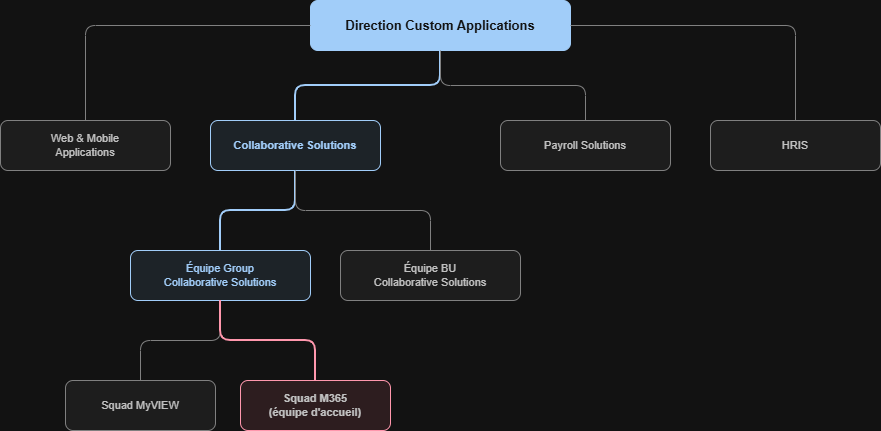
\includegraphics[width=\textwidth]{org_squads.png}
  \caption{Positionnement du squad M365 au sein de la direction Custom
    Applications.}
  \label{fig:org-squads}
\end{figure}

L'équipe fonctionne selon une approche agile, rythmée par plusieurs rituels au
cours de la semaine. Chaque jour, un daily réunit le squad pour faire le point
sur le travail de la veille, celui du jour, et remonter d'éventuels points
bloquants. Le lundi, un point d'équipe rassemble l'ensemble de l'équipe Group
Collaborative Solutions afin de coordonner les travaux entre les deux squads.
Le mardi, un point de squad se concentre sur l'avancement propre au squad M365.
Enfin, le vendredi, un point technique avec le référent technique, Nathan,
permet de valider les choix techniques et de discuter en profondeur des sujets
de conception avant leur mise en œuvre. Le suivi des tâches s'effectue tout au
long de la semaine dans Wrike, où le travail est formalisé et priorisé, ce qui
assure la traçabilité des développements et une visibilité partagée sur
l'avancement.

\begin{table}[H]
  \centering
  \caption{Rituels agiles suivis durant le stage.}
  \label{tab:rituels}
  \begin{tabularx}{\textwidth}{>{\bfseries}p{3.2cm} p{2.6cm} X}
    \toprule
    \normalfont\bfseries Rituel & \bfseries Fréquence & \bfseries Objectif \\
    \midrule
    Daily          & Quotidienne & Point sur la veille et la journée à venir,
                                   remontée des points bloquants \\
    Point d'équipe & Hebdo (lundi) & Coordination à l'échelle de l'équipe
                                     Group Collaborative Solutions \\
    Point de squad & Hebdo (mardi) & Suivi de l'avancement au sein du
                                     squad M365 \\
    Point technique & Hebdo (vendredi) & Validation des choix techniques avec
                                         le référent technique \\
    \bottomrule
  \end{tabularx}
\end{table}
\section{Environnement technique}
\label{sec:environnement-technique}
Les développements s'appuient sur une pile technique full-stack cohérente avec
celle du service, complétée par des outils de gestion de code, de suivi de
projet et d'assistance au développement.

\begin{table}[H]
  \centering
  \caption{Environnement technique du stage.}
  \label{tab:stack}
  \begin{tabularx}{\textwidth}{>{\bfseries}p{3.8cm} X}
    \toprule
    \normalfont\bfseries Catégorie & \bfseries Technologies et outils \\
    \midrule
    Back-end          & C\#, ASP.NET~Core (.NET~Core / .NET~Framework) \\
    Front-end         & Angular \\
    Base de données   & Microsoft SQL~Server \\
    Cloud             & Microsoft Azure (services cloud, Azure~AD) \\
    Gestion de code   & GitLab (instance auto-hébergée en interne) \\
    Gestion de projet & Wrike \\
    Assistance IA     & GitHub~Copilot (seul outil d'IA autorisé) \\
    Rédaction du rapport & Latex via la plateforme Overleaf~\cite{overleaf} \\
    \bottomrule
  \end{tabularx}
\end{table}
Ce socle est représentatif des projets du service~: un back-end .NET exposant
des services consommés par un front-end Angular, une persistance sur SQL~Server
et une intégration à l'écosystème Microsoft~365 et Azure. Il constitue le cadre
technique dans lequel s'inscrit la refonte de \csbag, présentée au
chapitre~\ref{chap:csbag}.
\chapter{État de l'art}
\label{chap:etat-art}

Avant d'aborder la conception de \csbag, ce chapitre dresse un état de l'art des
technologies, méthodes et bonnes pratiques disponibles à l'entrée en stage. Il
ne décrit pas mes réalisations, présentées au chapitre suivant, mais le cadre
existant dans lequel s'inscrit mon travail~: l'écosystème Microsoft, les
services cloud Azure, l'architecture des applications web modernes, la
conception des bases de données relationnelles et, enfin, les stratégies de
modernisation d'un existant. Chacune de ces notions servira ensuite de grille de
lecture pour analyser et justifier les choix techniques du
chapitre~\ref{chap:travaux}.

\section{L'écosystème Microsoft 365 et SharePoint}
\label{sec:m365}

Le service qui m'a accueilli développe ses solutions autour de Microsoft~365,
une suite d'outils collaboratifs hébergés dans le cloud~\cite{ms_m365}. Au cœur
de cette suite, SharePoint~Online est une plateforme de collaboration et de
gestion documentaire organisée en sites, chaque site regroupant des listes
(données structurées) et des bibliothèques de documents~\cite{ms_sharepoint}.
Dans un groupe fortement décentralisé, ce type de plateforme fournit un socle
commun à des centaines d'entités, ce qui explique sa place centrale au sein du
service.

Plusieurs approches permettent d'accéder par programme aux données de
Microsoft~365 et de SharePoint. Microsoft~Graph constitue l'interface REST
unifiée et recommandée aujourd'hui par Microsoft pour l'ensemble des services
de la suite~\cite{ms_graph}. À côté, deux approches plus anciennes subsistent~:
le modèle objet client (CSOM), spécifique à SharePoint, et l'API REST propre à
SharePoint~\cite{ms_sp_access}.

\begin{table}[H]
  \centering
  \caption{Approches d'accès programmatique à SharePoint~/ Microsoft~365.}
  \label{tab:sp-acces}
  \begin{tabularx}{\textwidth}{>{\bfseries}p{3.4cm} X p{2.9cm}}
    \toprule
    \normalfont\bfseries Approche & \bfseries Description & \bfseries Positionnement \\
    \midrule
    Microsoft Graph & Interface REST unifiée pour tout Microsoft~365
      (utilisateurs, fichiers, sites, etc.) & Approche moderne recommandée \\
    CSOM & Modèle objet côté client, spécifique à SharePoint & Approche
      historique \\
    API REST SharePoint & Accès REST propre à SharePoint & Approche historique \\
    \bottomrule
  \end{tabularx}
\end{table}

\section{Le cloud et les services Azure}
\label{sec:azure}

L'informatique en nuage (\textit{cloud computing}) désigne la fourniture à la
demande de ressources informatiques par un fournisseur, selon un modèle où l'on
consomme un service au lieu d'héberger et d'administrer soi-même
l'infrastructure. La définition de référence, établie par le NIST, distingue
trois modèles de service~: l'infrastructure (IaaS), la plateforme (PaaS) et le
logiciel (SaaS)~\cite{nist2011cloud}. Microsoft~Azure est la plateforme cloud de
Microsoft~; elle propose un ensemble de services managés que l'on assemble selon
les besoins d'une application.

Plusieurs de ces services sont directement pertinents pour une application
d'entreprise. La gestion des identités et de l'authentification est assurée par
Microsoft~Entra~ID, anciennement Azure~Active~Directory, qui prend notamment en
charge l'authentification unique (SSO) via le protocole OpenID~Connect
\cite{ms_entra,ms_oidc}. La protection des données sensibles repose sur
Azure~Key~Vault, un service dédié au stockage centralisé et sécurisé des secrets,
clés et certificats~\cite{ms_keyvault}~; cette approche répond à une bonne
pratique élémentaire, qui consiste à ne jamais inscrire de secret en clair dans
le code source. Enfin, l'exécution de traitements en arrière-plan peut s'appuyer
sur les Azure~WebJobs, déclenchés notamment par une file d'attente
Azure~Storage~Queue, ce qui permet de découpler et de fiabiliser des traitements
asynchrones~\cite{ms_webjobs}.

\begin{figure}[H]
  \centering
  \resizebox{0.95\textwidth}{!}{%
  \begin{tikzpicture}[
    font=\small,
    app/.style={rounded corners=5pt, draw=vinciblue, line width=1pt, fill=vinciblue!6,
      drop shadow={opacity=0.18,shadow xshift=1pt,shadow yshift=-1pt},
      align=center, text width=4cm, minimum height=1.3cm},
    serv/.style={rounded corners=5pt, draw=azurblue!70, line width=0.9pt, fill=white,
      drop shadow={opacity=0.16,shadow xshift=1pt,shadow yshift=-1pt},
      align=center, text width=2.8cm, minimum height=2.4cm, inner sep=4pt},
    conn/.style={-{Stealth[length=2.5mm]}, line width=1pt, azurblue!80}
  ]
    \node[app] (app) {\textbf{Application}\\[2pt]\footnotesize ASP.NET Core + Angular};
    \node[serv, below=2.4cm of app, xshift=-4.9cm] (entra) {};
    \node[serv, right=0.4cm of entra] (kv) {};
    \node[serv, right=0.4cm of kv] (queue) {};
    \node[serv, right=0.4cm of queue] (wj) {};
    % Entra ID : bouclier
    \begin{scope}[shift={([yshift=-0.5cm]entra.north)}]
      \fill[azurblue] (0,0.28) -- (0.22,0.17) -- (0.22,-0.07)
        .. controls (0.22,-0.26) and (0,-0.35) .. (0,-0.35)
        .. controls (0,-0.35) and (-0.22,-0.26) .. (-0.22,-0.07)
        -- (-0.22,0.17) -- cycle;
      \draw[white, line width=1pt] (-0.08,-0.02) -- (-0.01,-0.11) -- (0.1,0.09);
    \end{scope}
    \node[align=center] at ([yshift=-1.5cm]entra.north)
      {\textbf{\footnotesize Entra ID}\\[1pt]\rrole{Authentification \& SSO}\\\rrole{(OpenID Connect)}};
    % Key Vault : clé
    \begin{scope}[shift={([yshift=-0.5cm]kv.north)}]
      \draw[azurblue, line width=1.4pt] (-0.1,0) circle (0.11);
      \draw[azurblue, line width=1.4pt] (0.01,0) -- (0.28,0);
      \draw[azurblue, line width=1.4pt] (0.2,0) -- (0.2,-0.1);
      \draw[azurblue, line width=1.4pt] (0.28,0) -- (0.28,-0.12);
    \end{scope}
    \node[align=center] at ([yshift=-1.5cm]kv.north)
      {\textbf{\footnotesize Key Vault}\\[1pt]\rrole{Secrets, clés}\\\rrole{et certificats}};
    % Queue : messages empilés
    \begin{scope}[shift={([yshift=-0.45cm]queue.north)}]
      \foreach \y in {0.14,0.0,-0.14} {
        \draw[azurblue, line width=0.9pt, rounded corners=1pt] (-0.24,\y-0.045) rectangle (0.24,\y+0.045);}
    \end{scope}
    \node[align=center] at ([yshift=-1.5cm]queue.north)
      {\textbf{\footnotesize Storage Queue}\\[1pt]\rrole{File d'attente}\\\rrole{de messages}};
    % WebJobs : engrenage
    \begin{scope}[shift={([yshift=-0.5cm]wj.north)}]
      \draw[azurblue, line width=1.2pt] (0,0) circle (0.12);
      \foreach \a in {0,45,...,315} \draw[azurblue, line width=1.8pt] (\a:0.12) -- (\a:0.2);
      \fill[azurblue] (0,0) circle (0.04);
    \end{scope}
    \node[align=center] at ([yshift=-1.5cm]wj.north)
      {\textbf{\footnotesize WebJobs}\\[1pt]\rrole{Traitements}\\\rrole{en arrière-plan}};
    % connexions
    \draw[conn] (app.south) .. controls +(0,-0.6) and +(0,0.6) .. (entra.north)
       node[pos=0.5, sloped, above, font=\scriptsize\itshape, text=grisfonce]{s'authentifie};
    \draw[conn] (app.south) .. controls +(0,-0.6) and +(0,0.6) .. (kv.north)
       node[pos=0.55, right, font=\scriptsize\itshape, text=grisfonce]{lit les secrets};
    \draw[conn] (queue.east) -- node[above, font=\scriptsize\itshape, text=grisfonce]{déclenche} (wj.west);
    % cadre
    \begin{scope}[on background layer]
      \node[draw=azurblue!35, line width=0.8pt, rounded corners=6pt, fill=azurblue!4,
            fit=(entra)(wj), inner sep=11pt] (box) {};
    \end{scope}
    \node[anchor=west, font=\footnotesize\bfseries, text=azurblue]
      at ([xshift=5pt,yshift=-2pt]box.north west) {Services Azure managés};
  \end{tikzpicture}%
  }
  \caption{Services Azure managés et leur rôle autour d'une application.}
  \label{fig:azure}
\end{figure}

\section{L'architecture des applications web modernes}
\label{sec:archi-web}

Les applications web ont longtemps reposé sur un modèle multipage, où le serveur
renvoie une page HTML complète à chaque interaction. Le modèle dominant
aujourd'hui est celui de l'application monopage (\textit{Single Page
Application}, SPA)~: une seule page est chargée initialement, puis mise à jour
dynamiquement côté navigateur, le serveur n'échangeant plus que des données. Ces
échanges s'appuient sur une API REST, style d'architecture formalisé par
Fielding, fondé sur la manipulation de ressources via les verbes du protocole
HTTP~\cite{fielding2000rest}. Ce découplage entre un front-end autonome et une
API back-end permet de développer et de faire évoluer les deux indépendamment,
et d'ouvrir l'API à d'autres consommateurs. Dans l'écosystème considéré, ce
modèle se traduit par un front-end Angular~\cite{angular_docs} dialoguant avec
une API ASP.NET~Core~\cite{ms_aspnetcore}.

\begin{figure}[H]
  \centering
  \begin{tikzpicture}[
    font=\footnotesize,
    card/.style={rounded corners=3pt, draw=vinciblue, line width=0.8pt, fill=white,
      align=center, text width=5.2cm, minimum height=0.8cm},
    layer/.style={rounded corners=2pt, draw=vinciblue!55, line width=0.6pt,
      fill=vinciblue!8, align=center, text width=4.8cm, minimum height=0.6cm},
    flow/.style={-{Stealth[length=2.2mm]}, line width=0.9pt, vinciblue},
    tag/.style={rounded corners=2pt, draw=vincired!55, fill=vincired!7,
      font=\scriptsize, text=grisfonce, align=center, inner sep=2pt},
    lbl/.style={font=\scriptsize\itshape, text=grisfonce, fill=white, inner sep=1pt}
  ]
    % Front-end
    \node[card] (spa) {\textbf{Navigateur} — Angular (SPA)};
    % Couches API
    \node[layer, below=1cm of spa] (ctrl) {Contrôleurs (présentation)};
    \node[layer, below=0.2cm of ctrl] (svc) {Services (métier)};
    \node[layer, below=0.2cm of svc] (repo) {Repositories (accès données)};
    \draw[flow] (ctrl) -- (svc);
    \draw[flow] (svc) -- (repo);
    % Cadre API
    \begin{scope}[on background layer]
      \node[draw=vinciblue, line width=0.8pt, rounded corners=4pt, fill=grisclair,
            fit=(ctrl)(svc)(repo), inner sep=8pt] (api) {};
    \end{scope}
    \node[anchor=south west, font=\scriptsize\bfseries, text=vinciblue]
          at ([xshift=2pt,yshift=1pt]api.north west) {API ASP.NET Core};
    % Tags patrons
    \node[tag, right=0.4cm of ctrl] (t1) {DTO};
    \node[tag, right=0.4cm of repo] (t2) {Repository};
    \draw[vincired!55, dotted, line width=0.6pt] (ctrl.east) -- (t1.west);
    \draw[vincired!55, dotted, line width=0.6pt] (repo.east) -- (t2.west);
    % Base de données
    \node[cylinder, shape border rotate=90, aspect=0.3, draw=vincired,
          line width=0.8pt, fill=vincired!8, minimum width=2cm, minimum height=0.9cm,
          align=center, below=1cm of api] (db) {\textbf{SQL Server}};
    % Flèches principales
    \draw[flow] (spa) -- node[lbl,right]{HTTP / REST (JSON)} (api.north);
    \draw[flow] (api.south) -- node[lbl,right]{Entity Framework Core} (db);
  \end{tikzpicture}
  \caption{Architecture en couches d'une application web moderne~: du front-end
    SPA à la base de données relationnelle.}
  \label{fig:archi}
\end{figure}

Côté back-end, les applications d'entreprise s'organisent classiquement en
couches~: une couche de présentation (les contrôleurs qui reçoivent les
requêtes), une couche métier (les services qui portent la logique) et une couche
d'accès aux données. Cette organisation s'accompagne de plusieurs patrons de
conception éprouvés, recensés notamment par Fowler~\cite{fowler2002poeaa}. Le
patron Repository isole l'accès aux données derrière une interface~; l'Unit of
Work regroupe un ensemble de modifications au sein d'une même transaction~; les
objets de transfert de données (DTO) découplent les entités internes de ce que
l'API expose. À cela s'ajoute l'injection de dépendances, principe qui consiste
à fournir à un composant les services dont il a besoin plutôt que de les laisser
les instancier lui-même, ce qui améliore la testabilité et le découplage
\cite{seemann2019di,ms_di}.

L'accès aux données relationnelles s'appuie fréquemment sur un
\textit{mapping} objet-relationnel (ORM), qui traduit automatiquement entre les
objets du langage et les tables de la base. Entity~Framework~Core est l'ORM de
référence de l'écosystème .NET~\cite{ms_efcore}. Un ORM accélère le
développement et réduit le code répétitif, au prix d'un contrôle plus fin qu'offre
en contrepartie l'accès direct par requêtes (ADO.NET), parfois préféré pour les
traitements les plus sensibles à la performance.

\section{Les bases de données relationnelles et la normalisation}
\label{sec:normalisation}

Le modèle relationnel, introduit par Codd, organise les données en relations
(tables) reliées entre elles, et constitue le fondement des systèmes de gestion
de bases de données actuels~\cite{codd1970relational}. La qualité d'un schéma
relationnel repose en grande partie sur sa normalisation, c'est-à-dire son
organisation en formes normales successives (1NF, 2NF, 3NF) visant à éliminer la
redondance des données~\cite{codd1972normalization}.

L'enjeu de la normalisation est concret. Lorsqu'une même information est dupliquée
en plusieurs endroits, par exemple une valeur saisie en texte libre répétée sur
de nombreuses lignes, la base s'expose à des anomalies de mise à jour~: une
correction partielle laisse des incohérences, et les fautes de saisie créent de
faux doublons~\cite{elmasri2016fundamentals}. La normalisation répond à ce
problème en extrayant les données répétées dans des tables de référence
dédiées. Les relations de type plusieurs-à-plusieurs sont alors modélisées par
des tables d'association, qui relient deux entités et peuvent porter des
attributs propres à la relation~\cite{silberschatz2019database}. Ces principes
constituent la grille de lecture qui servira, au chapitre~\ref{chap:travaux}, à
analyser le schéma existant et à justifier son évolution.

\section{Dette technique et modernisation applicative}
\label{sec:dette-technique}

Toute application vit et évolue. Les lois de l'évolution logicielle énoncées par
Lehman rappellent qu'un logiciel utilisé doit être continuellement adapté, sous
peine de voir son utilité décroître, et que sa complexité tend à augmenter avec
le temps si aucun effort n'est consenti pour la maîtriser~\cite{lehman1980evolution}.
Cette dégradation progressive est captée par la notion de dette technique,
métaphore introduite par Cunningham~: privilégier une solution rapide à une
solution propre revient à contracter une dette, qu'il faudra rembourser plus tard
sous forme d'efforts de maintenance accrus~\cite{cunningham1992wycash}.

Rembourser cette dette passe par le \textit{refactoring}, discipline formalisée
par Fowler, qui consiste à améliorer la structure interne d'un code sans en
modifier le comportement observable~\cite{fowler2018refactoring}. À l'échelle
d'une application entière, deux stratégies de modernisation s'opposent~: la
réécriture complète, qui repart de zéro mais concentre les risques, et la refonte
incrémentale, qui fait évoluer l'existant par étapes tout en le gardant
fonctionnel. Le patron \textit{Strangler~Fig} illustre cette seconde voie, où le
nouveau système remplace progressivement l'ancien~\cite{fowler2004strangler}.
Cette démarche progressive s'inscrit dans le cadre plus large de la maintenance
logicielle, notamment évolutive, telle que la décrivent les référentiels du génie
logiciel~\cite{iso14764}.

Ces bonnes pratiques, issues de la littérature, fournissent le cadre théorique
sur lequel s'appuie la suite du rapport. Le chapitre suivant confronte cet état
de l'art à l'existant de \csbag et présente, à sa lumière, la conception et la
réalisation de sa version~2.
% =====================================================================
%  CHAPITRE 4 - TRAVAUX RÉALISÉS
%  Méthodologie de travail + CS BAG v2 + Elium Sauvegarde + Access TTC
% =====================================================================
\chapter{Travaux réalisés}
\label{chap:travaux}

Ce chapitre présente d'abord la méthodologie de travail appliquée au sein du
service, puis détaille les trois projets sur lesquels j'ai travaillé~: la
refonte de \csbag, l'outil de sauvegarde Elium et le système de rapports
d'accès TTC/GO.

% -----------------------------------------------------------------
\section{Méthodologie de travail au sein de VESI}
\label{sec:methodologie}

Chaque évolution applicative suit un processus structuré en plusieurs étapes,
depuis l'expression du besoin jusqu'à la mise en production et le suivi.
La figure~\ref{fig:workflow} synthétise ce cycle.

\begin{figure}[H]
  \centering
  \scalebox{0.82}{%
  \begin{tikzpicture}[
    font=\scriptsize,
    step/.style={rounded corners=2pt, draw=vinciblue, line width=0.6pt,
      fill=vinciblue!6, align=center, text width=3.2cm, minimum height=0.55cm,
      inner sep=2pt},
    arr/.style={-{Stealth[length=1.8mm]}, line width=0.7pt, vinciblue!80}
  ]
    % Colonne gauche (étapes 1-5)
    \node[step] (s1) {\textbf{1.} Spécifications\\(analyste fonctionnel)};
    \node[step, below=0.2cm of s1] (s2) {\textbf{2.} Réunion de cadrage\\(AF + chef de projet)};
    \node[step, below=0.2cm of s2] (s3) {\textbf{3.} Développement\\(environnement local)};
    \node[step, below=0.2cm of s3] (s4) {\textbf{4.} Déploiement DEV\\(ressources Azure)};
    \node[step, below=0.2cm of s4] (s5) {\textbf{5.} Tests développeur\\(environnement DEV)};
    % Colonne droite (étapes 6-10)
    \node[step, right=1cm of s1] (s10) {\textbf{10.} Monitoring};
    \node[step, below=0.2cm of s10] (s9) {\textbf{9.} Mise en production};
    \node[step, below=0.2cm of s9] (s8) {\textbf{8.} Tests finaux (AF)\\+ validation};
    \node[step, below=0.2cm of s8] (s7) {\textbf{7.} Corrections\\des retours};
    \node[step, below=0.2cm of s7] (s6) {\textbf{6.} Mise en recette\\+ tests AF};
    % Flèches colonne gauche
    \draw[arr] (s1) -- (s2);
    \draw[arr] (s2) -- (s3);
    \draw[arr] (s3) -- (s4);
    \draw[arr] (s4) -- (s5);
    % Transition gauche -> droite
    \draw[arr] (s5.east) -- ++(0.2,0) |- (s6.west);
    % Flèches colonne droite (remonte)
    \draw[arr] (s6) -- (s7);
    \draw[arr] (s7) -- (s8);
    \draw[arr] (s8) -- (s9);
    \draw[arr] (s9) -- (s10);
  \end{tikzpicture}%
  }
  \caption{Cycle de réalisation d'un lot applicatif au sein de VESI.}
  \label{fig:workflow}
\end{figure}

\begin{enumerate}[leftmargin=*, nosep]
  \item \textbf{Spécifications fonctionnelles}~: l'analyste fonctionnel rédige
    un document de spécifications détaillé pour chaque lot, décrivant les règles
    métier, les maquettes d'écran et les critères d'acceptation.
  \item \textbf{Réunion de cadrage}~: l'analyste fonctionnel et le chef de
    projet présentent le document à l'équipe de développement lors d'une réunion
    dédiée, au cours de laquelle les questions techniques sont levées.
  \item \textbf{Développement et conception}~: le développeur implémente la
    solution sur son environnement local (machine personnelle), en respectant
    l'architecture et les conventions du projet.
  \item \textbf{Déploiement en environnement DEV}~: le code est déployé sur les
    ressources Azure de l'environnement de développement (App~Service, base de
    données, Key~Vault, etc.).
  \item \textbf{Tests développeur}~: le développeur vérifie le bon
    fonctionnement dans l'environnement DEV, en testant les scénarios décrits
    dans les spécifications.
  \item \textbf{Mise en recette}~: une fois les tests développeur validés, le
    code est déployé en environnement de recette. L'analyste fonctionnel réalise
    ses propres tests et constitue un répertoire de retours (captures d'écran,
    vidéos) documentant les anomalies et écarts constatés.
  \item \textbf{Correction des retours}~: le développeur corrige les anomalies
    signalées et effectue un nouveau cycle de tests.
  \item \textbf{Tests finaux et validation}~: l'analyste fonctionnel valide les
    corrections en recette. Cette étape conditionne le passage en production.
  \item \textbf{Mise en production}~: le code validé est déployé sur
    l'environnement de production, accessible aux utilisateurs finaux.
  \item \textbf{Monitoring}~: l'équipe surveille l'application en production
    (journaux, alertes, retours utilisateurs) pour détecter d'éventuelles
    régressions.
\end{enumerate}

Ce processus a été appliqué à chacun des lots de \csbag ainsi qu'aux autres
projets présentés ci-après.

% =================================================================
\section{\csbag v2 : conception et réalisation}
\label{sec:csbag}

\subsection{L'existant : \csbag v1 et ses limites}
\label{sec:existant}
% >>> À RÉDIGER <<<

\subsection{Expression des besoins et exigences}
\label{sec:besoins}
% >>> À RÉDIGER <<<

\subsection{Architecture cible}
\label{sec:architecture}
% >>> À RÉDIGER <<<

\subsection{Modèle de données et migration}
\label{sec:donnees-migration}
% >>> À RÉDIGER <<<

\subsection{Réalisation}
\label{sec:realisation}
% >>> À RÉDIGER <<<

\subsection{Qualité, tests et déploiement}
\label{sec:qualite}
% >>> À RÉDIGER <<<

\subsection{Résultats}
\label{sec:resultats-csbag}
% >>> À RÉDIGER <<<

% =================================================================
\section{Elium Sauvegarde}
\label{sec:elium}

Le service Collaborative Solutions utilise la plateforme Elium comme base de
connaissances interne. Afin de prévenir toute perte de contenu et de centraliser
l'information dans l'écosystème SharePoint, un outil de synchronisation
automatique a été développé.

\subsection{Objectif et besoin}
\label{sec:elium-objectif}

L'outil \textit{Elium Sauvegarde} est une application console .NET~6 dont le
rôle est de répliquer les articles (\textit{stories}) publiés sur Elium vers des
pages SharePoint~Online. Il supporte deux modes de synchronisation~: un mode
complet (toutes les stories) et un mode incrémental (basé sur une fenêtre de
jours configurable), permettant une exécution planifiée régulière.

\subsection{Fonctionnement technique}
\label{sec:elium-technique}

Le processus de synchronisation se déroule en plusieurs étapes~:
\begin{enumerate}[nosep]
  \item lecture des éléments de référence existants sur le site SharePoint cible~;
  \item récupération des stories depuis l'API Elium~;
  \item calcul des différences (stories supprimées, modifiées, nouvelles)~;
  \item suppression des pages SharePoint obsolètes et de leurs entrées en liste~;
  \item création et publication des nouvelles pages~;
  \item journalisation détaillée des résultats (succès et erreurs).
\end{enumerate}

L'application s'appuie sur Azure~Key~Vault pour la gestion des secrets
(jetons d'API, certificats) et utilise Microsoft~Graph pour l'interaction avec
SharePoint.

\subsection{Résultats}
\label{sec:elium-resultats}
% >>> À RÉDIGER <<<

% =================================================================
\section{Rapports d'accès TTC/GO}
\label{sec:ttcgo}

La gouvernance des accès aux ressources partagées (sites SharePoint, partages
de fichiers) est un enjeu majeur pour un groupe décentralisé comme VINCI~Energies.
Le projet \textit{Access~Report~TTC/GO} automatise la génération de ces rapports
de permissions.

\subsection{Objectif et besoin}
\label{sec:ttcgo-objectif}

Ce système repose sur plusieurs Azure~WebJobs qui traitent des demandes de
rapports d'accès. Un job de gouvernance alimente des files d'attente
(Azure~Storage~Queue) avec les demandes entrantes, puis des jobs spécialisés
(TTC, GO, fichiers BU, confidentiels) exécutent les exports de permissions
correspondants.

\subsection{Fonctionnement technique}
\label{sec:ttcgo-technique}

Le traitement d'une demande suit le parcours suivant~:
\begin{enumerate}[nosep]
  \item réception d'une requête depuis la file de gouvernance~;
  \item vérification des doublons et des demandes déjà traitées~;
  \item export des permissions (NTFS ou SharePoint selon le périmètre)~;
  \item génération d'un rapport Excel~;
  \item envoi du rapport par courriel (en pièce jointe ou via un lien de
    partage pour les fichiers volumineux)~;
  \item journalisation de l'exécution en base SQL~Server.
\end{enumerate}

L'application utilise le SDK Azure~WebJobs avec des déclencheurs sur file
d'attente et sur minuteur, Azure~Key~Vault pour les secrets, et
Application~Insights pour le monitoring.

\subsection{Résultats}
\label{sec:ttcgo-resultats}
% >>> À RÉDIGER <<<

% =====================================================================
%  CHAPITRE 5 - MISSIONS TRANSVERSES  (~3 pages)
% =====================================================================
\chapter{Missions transverses}
\label{chap:transverses}

% >>> À RÉDIGER <<< (migration BDD, Azure, autres sujets ponctuels)

% =====================================================================
%  CHAPITRE 5 - RECUL SUR LE STAGE
% =====================================================================
\chapter{Recul sur le stage}
\label{chap:recul}

Après avoir détaillé les travaux réalisés, ce chapitre prend du recul sur ce que
cette expérience m'a réellement apporté. Il ne revient pas sur les solutions
techniques mises en \oe uvre, mais sur la manière dont ma façon de travailler a
évolué, sur les compétences que j'ai construites et sur celles qu'il me reste à
approfondir.

\section{Apports techniques}
\label{sec:apports-techniques}

L'apport le plus déterminant du stage tient moins aux technologies employées
qu'à la nature du terrain sur lequel j'ai travaillé. Jusqu'ici, mes projets
étaient conçus depuis une page blanche~: je définissais moi-même le modèle de
données, l'architecture et les conventions, et le résultat était évalué à sa
livraison. \csbag m'a placé dans la situation inverse. J'ai hérité d'une
application en service, avec des données réelles saisies pendant plusieurs
années, des choix antérieurs que je n'avais pas faits, et des utilisateurs qui
continuaient à s'en servir pendant que je la modifiais. La question n'est alors
jamais seulement « quelle est la bonne conception~? », mais « comment atteindre
la bonne conception sans casser ce qui fonctionne~? ». La refonte du modèle de
données l'a illustré avec le plus de force~: je connaissais les formes normales
en théorie, j'ignorais ce que représente concrètement leur application sur des
données déjà dégradées. Lors de la migration~V019, les doublons présents en base
empêchaient la création des clés primaires, et il a fallu nettoyer avant de
contraindre, situation qu'un exercice académique, où les données sont propres
par construction, ne permet pas de rencontrer. J'en ai retiré une conviction
durable~: la qualité d'un modèle de données ne se juge pas sur son schéma, mais
sur ce qu'il rend possible ou impossible aux utilisateurs. Un champ de texte
libre ne produit pas immédiatement de bug~; il produit, au bout de quelques
années, un inventaire sur lequel plus aucun filtre n'est fiable. C'est également
l'analyse en amont qui m'a le plus fait progresser~: prendre le temps de
requêter les données réelles avant de coder m'a permis de formuler un problème
que personne n'avait exprimé, et de le documenter suffisamment pour qu'il soit
accepté.

La migration du socle technique m'a appris une autre forme de rigueur. Le
réflexe naturel aurait été de sauter directement d'Angular~14 à Angular~20~; le
choix d'une progression palier par palier, plus long, m'a montré la valeur d'une
méthode qui isole les causes de régression au lieu de les cumuler. Plus
largement, j'ai découvert que la maintenance d'un socle n'est pas une tâche
secondaire mais une condition de la sécurité de l'application, puisqu'une
version sortie du support ne reçoit plus aucun correctif.

Les interventions sur Elium Sauvegarde et Access Report TTC~GO ont
considérablement fait évoluer ma manière de diagnostiquer un problème. Dans les
deux cas, l'application ne produisait aucune erreur~: Elium échouait
globalement à cause d'une anomalie sur un seul article, et Access Report livrait
des rapports incomplets sans qu'aucune trace ne soit journalisée. J'ai appris à
me méfier de l'absence de message d'erreur, à raisonner par élimination plutôt
qu'à modifier le code au hasard, et surtout à ne pas m'arrêter au premier
symptôme corrigé. Sur Access Report, la distinction entre le contournement mis
en place pour débloquer rapidement l'exploitation et la correction de fond
apportée ensuite à la bibliothèque partagée m'a fait comprendre qu'un correctif
a une portée~: résoudre le problème pour soi ou le résoudre pour tous ceux qui
utilisent le même composant ne demandent ni le même effort, ni le même niveau de
précaution. C'est aussi sur ces missions que j'ai mesuré l'importance de
l'observabilité~: un traitement qui ne dit rien de ce qu'il a fait est un
traitement que personne ne peut valider.

L'exigence de qualité imposée par la chaîne d'intégration continue a été, au
début, difficile à accepter. Voir une livraison bloquée pour une complexité
cognitive excessive ou pour une description manquante sur un tableau HTML m'a
d'abord semblé formaliste. J'ai progressivement compris que ces règles rendent
explicite une exigence que je n'appliquais jusqu'ici qu'au jugé, et qu'un code
qui passe ces contrôles est un code qu'un autre développeur pourra reprendre.
De la même façon, la découverte de la gestion des secrets et des mécanismes
d'autorisation m'a fait passer d'une conception défensive de la sécurité, où
l'on protège l'interface, à une conception plus juste, où l'on considère que
l'interface peut être contournée et que le contrôle doit exister côté serveur.

Sur le plan de l'autonomie, l'évolution a été nette. Les premières semaines,
je validais chaque orientation avant de l'engager. À partir du deuxième lot,
j'arrivais aux points techniques avec une proposition argumentée et ses
alternatives, et la discussion portait sur le choix plutôt que sur la direction
à prendre. Cette autonomie reste toutefois inégale selon les domaines~: je suis
aujourd'hui à l'aise sur la conception applicative et la donnée, nettement
moins sur les aspects d'exploitation, où j'ai surtout observé et exécuté des
procédures existantes.

\section{Apports humains et organisationnels}
\label{sec:apports-humains}

Avant ce stage, ma représentation du travail en équipe reposait sur les projets
tuteurés~: un groupe d'étudiants au même niveau, un objectif commun, et une
répartition des tâches décidée entre pairs. L'équipe que j'ai rejointe
fonctionne autrement. Chacun y occupe un rôle défini, avec des attentes et une
temporalité propres, et une part importante du travail consiste à s'articuler
avec les autres plutôt qu'à avancer seul. J'ai dû apprendre à identifier le bon
interlocuteur selon la question~: le chef de projet pour un arbitrage de
périmètre, le référent technique pour une orientation de conception, l'analyste
fonctionnelle pour lever une ambiguïté dans une spécification.

La relation avec l'analyste fonctionnelle a été particulièrement formatrice.
Recevoir un cahier de retours documenté après chaque mise en recette m'a
d'abord été inconfortable~: un écran que je considérais comme terminé revenait
avec une liste d'anomalies. J'ai compris assez vite que ces retours ne portaient
pas un jugement sur mon travail, mais sur l'écart entre ce que j'avais compris
du besoin et ce qui était attendu. Cette prise de conscience a modifié ma façon
de travailler en amont~: j'ai pris l'habitude de reformuler les points ambigus
dès la réunion de cadrage plutôt que de les interpréter, ce qui a réduit le
nombre d'allers-retours au fil des lots.

Le moment le plus structurant du stage a été celui où j'ai présenté à l'équipe
mon diagnostic de l'existant et proposé d'élargir le périmètre de la mission.
Il ne suffisait pas d'avoir raison techniquement~: il fallait démontrer que ces
chantiers, absents des spécifications, conditionnaient la valeur des
fonctionnalités demandées, et que le coût supplémentaire était justifié. J'ai
appris à formuler un problème technique dans des termes compréhensibles par des
interlocuteurs qui n'allaient pas lire le code, en m'appuyant sur des exemples
concrets tirés des données réelles plutôt que sur des principes de conception.
C'est probablement la compétence la plus transférable que j'ai développée.

Les rituels agiles ont eu un effet que je n'avais pas anticipé. Le point
quotidien oblige à rendre son travail intelligible en quelques phrases, et à
signaler un blocage au lieu de s'obstiner~: j'ai mis plusieurs semaines à
accepter que remonter une difficulté rapidement n'est pas un aveu de faiblesse,
mais le comportement attendu. Le point technique hebdomadaire, lui, m'a habitué
à défendre un choix devant quelqu'un de plus expérimenté, et à distinguer une
critique de ma solution d'une critique de mon travail.

Le fait de mener trois applications en parallèle, sur des piles techniques et
des problématiques différentes, m'a confronté à la gestion des priorités.
Basculer d'une évolution fonctionnelle planifiée vers un incident remonté par un
utilisateur suppose d'accepter de suspendre une tâche en cours, ce que je
faisais mal au départ~: j'avais tendance à vouloir terminer avant de changer de
sujet, y compris lorsque l'urgence justifiait l'inverse. Le suivi formalisé des
tâches et les échanges avec le chef de projet m'ont aidé à hiérarchiser selon
l'impact plutôt que selon mon confort.

Enfin, la participation aux réunions concernant d'autres projets du service, aux
mises en production de renouvellement de secrets et au traitement des problèmes
remontés par les utilisateurs m'a donné une vision que le seul développement ne
m'aurait pas apportée. J'ai découvert qu'une application vit bien plus longtemps
qu'elle n'est développée, et qu'une part significative du travail d'une équipe
consiste à maintenir en condition opérationnelle ce qui existe déjà. Cela a
modifié ma manière de concevoir~: je me demande désormais, en écrivant une
fonctionnalité, comment elle sera diagnostiquée le jour où elle
dysfonctionnera.

\section{Lien avec la formation ENSIM}
\label{sec:lien-ensim}

Plusieurs enseignements suivis à l'ENSIM se sont révélés directement
mobilisables, mais rarement sous la forme dans laquelle je les avais appris.

Le cours de bases de données relationnelles est celui dont l'apport a été le
plus direct. La modélisation et les formes normales m'ont fourni le cadre
d'analyse qui m'a permis de qualifier le problème du modèle existant, et de
proposer une solution argumentée plutôt qu'une intuition. Ce que le stage a
ajouté, c'est la dimension temporelle et opérationnelle que l'exercice
académique ignore~: normaliser une base vide est un problème de conception,
normaliser une base en production est un problème de migration, qui suppose des
scripts réversibles, des contrôles préalables et une reprise des données
existantes.

Le génie logiciel, la conception objet et le développement web ont constitué le
socle de mon travail sur l'architecture en couches de l'application. La
séparation des responsabilités, la notion de contrat entre composants et les
patrons de conception vus en cours m'ont permis de me repérer rapidement dans
une base de code que je n'avais pas écrite, et l'architecture n-tiers étudiée en
formation s'est concrétisée dans le découpage réel de la solution, en projets
distincts dont chacun a une responsabilité assignée. Je n'avais pratiqué ni
Angular ni~.NET avant le stage~; c'est la compréhension de ces concepts
sous-jacents, plutôt que la connaissance d'un framework particulier, qui m'a
permis de monter en compétence sans blocage majeur, ce qui confirme l'intérêt
d'une formation qui enseigne des principes plutôt que des outils. Le stage m'a
appris en revanche ce qui s'enseigne difficilement en cours~: qu'une
architecture existante porte des compromis, et qu'un développeur qui la reprend
doit d'abord comprendre pourquoi ces compromis ont été faits avant de les
corriger.

Ma spécialité, Interaction Personnes Systèmes, a trouvé une application moins
attendue mais réelle. La dette ergonomique identifiée dans l'application
existante, l'absence de retour visuel pendant les chargements, la difficulté à
retrouver une information dans de longues listes, relève exactement des
questions traitées en formation. Le travail sur la lisibilité de l'historique
des actions en est l'exemple le plus net~: le problème n'était pas de tracer les
modifications, mais de les présenter à une granularité compréhensible pour
l'utilisateur plutôt qu'à celle du système. Les exigences d'accessibilité
remontées par les analyses de qualité ont, de la même manière, prolongé une
sensibilité acquise en cours.

Les enseignements de gestion de projet et de méthodes agiles m'ont permis
d'arriver en connaissant le vocabulaire et la logique des rituels. Leur pratique
quotidienne m'a toutefois appris quelque chose que le cours ne transmet pas~:
l'agilité en entreprise n'est pas un cadre appliqué à la lettre, mais une
organisation ajustée à la réalité d'une équipe, avec des rituels dont chacun
a une fonction précise.

Trois domaines ont en revanche mis en évidence un écart réel entre ma formation
et le terrain. Le cloud, d'abord~: si les notions de réseaux et de systèmes
m'ont aidé à comprendre les mécanismes sous-jacents, je n'avais aucune pratique
d'une plateforme comme Azure, et j'ai dû acquérir en autonomie la logique des
services managés, de l'authentification par certificat et de la séparation des
environnements. La mise en production, ensuite~: c'est probablement l'écart le
plus important, car aucun projet académique ne m'avait confronté à l'idée qu'une
erreur ne se corrige pas par une nouvelle exécution du programme, mais engage
des données et des utilisateurs réels. La montée de version d'un socle
technique, enfin, est une opération que je n'avais jamais eu l'occasion de
pratiquer, et dont j'ignorais qu'elle constitue une activité à part entière du
métier.

Ce stage m'a également révélé deux compétences qu'il me reste à construire. La
première concerne les tests automatisés~: l'application dont j'avais la charge
n'en disposait pas côté serveur, et j'ai validé mon travail par des tests
manuels et par la recette fonctionnelle. Cette situation m'a fait mesurer, par
son absence, ce qu'une couverture de tests apporte en confiance lors d'une
refonte, mais elle ne m'a pas permis d'en développer la pratique. La seconde
concerne le déploiement automatisé~: j'ai travaillé avec une chaîne
d'intégration continue qui compile et analyse le code, sans intervenir sur son
paramétrage, et les déploiements auxquels j'ai participé restaient largement
manuels. Ce sont les deux axes sur lesquels je souhaite progresser en priorité.

Au terme de cette expérience, ma représentation du métier d'ingénieur
développeur a changé. Je l'envisageais essentiellement comme une activité de
production de code~; je le comprends aujourd'hui comme un travail d'analyse et
d'arbitrage, où la difficulté réside moins dans l'écriture d'une solution que
dans l'identification du bon problème et dans la capacité à le formuler
suffisamment clairement pour qu'une équipe décide de le traiter.

% =====================================================================
%  CONCLUSION  (1 page)
%  Démarche + principaux résultats, courtes perspectives,
%  compétences personnelles mobilisées.
% =====================================================================
\chapter*{Conclusion}
\addcontentsline{toc}{chapter}{Conclusion}
\markboth{Conclusion}{Conclusion}

% >>> À RÉDIGER <<<
\textit{[Conclusion à rédiger.]}


% -------------------- BACKMATTER --------------------
% Références documentaires
\printbibliography[heading=bibintoc,title={Références documentaires}]

% Glossaire des acronymes
% =====================================================================
%  GLOSSAIRE DES ACRONYMES
% =====================================================================
\chapter*{Glossaire}
\addcontentsline{toc}{chapter}{Glossaire}
\markboth{Glossaire}{Glossaire}

\begin{description}[style=nextline,leftmargin=3cm,labelwidth=2.8cm]
  \item[ADM] Compte d'administration (Administration Account)
  \item[API] Application Programming Interface
  \item[BDD] Base de données
  \item[BU] Business Unit
  \item[CI/CD] Continuous Integration / Continuous Deployment
  \item[CSOM] Client-Side Object Model (modèle objet côté client SharePoint)
  \item[CS BAG] Collaborative Solutions Bag
  \item[DEV] Environnement de développement
  \item[DTO] Data Transfer Object (objet de transfert de données)
  \item[EF Core] Entity Framework Core
  \item[ENSIM] École Nationale Supérieure d'Ingénieurs du Mans
  \item[ETP] Équivalent temps plein
  \item[HRIS] Human Resources Information System
  \item[IaaS] Infrastructure as a Service
  \item[ICT] Information and Communications Technology
  \item[MEP] Mise en production
  \item[M365] Microsoft 365
  \item[NIST] National Institute of Standards and Technology
  \item[ORM] Object-Relational Mapping (mapping objet-relationnel)
  \item[PaaS] Platform as a Service
  \item[PFE] Projet de Fin d'Études
  \item[QHSE] Qualité, Hygiène, Sécurité et Environnement
  \item[REST] Representational State Transfer
  \item[RSE] Responsabilité sociétale et environnementale
  \item[SaaS] Software as a Service
  \item[SIRH] Système d'information des ressources humaines
  \item[SPA] Single Page Application (application monopage)
  \item[SSO] Single Sign-On (authentification unique)
  \item[UAT] User Acceptance Testing (environnement de recette)
  \item[UPN] User Principal Name (identifiant utilisateur Azure)
  \item[URD] Universal Registration Document (document d'enregistrement universel)
  \item[VESI] VINCI Energies Systèmes d'Information
\end{description}


% Annexes
% =====================================================================
%  ANNEXES
%  Qualité rédactionnelle équivalente au texte principal.
%  Chaque annexe doit être référencée dans le corps du rapport.
% =====================================================================
\appendix
\chapter*{Annexes}
\addcontentsline{toc}{chapter}{Annexes}
\markboth{Annexes}{Annexes}

% Numérotation des annexes : A, B, C...
\renewcommand{\thesection}{\Alph{section}}
\setcounter{section}{0}
\titleformat{\section}
  {\normalfont\normalsize\bfseries\color{vinciblue}}{Annexe~\thesection}{1em}{}

\section{Évolution de l'interface de \csbag}
\label{ann:v1v2}

Les captures ci-dessous illustrent l'amélioration de l'ergonomie décrite en
section~\ref{sec:existant}. Pour chaque page, la version~1 (à gauche) est mise
en regard de la version~2 (à droite).

\subsection*{Page d'accueil}

\begin{figure}[H]
  \centering
  \begin{subfigure}[t]{0.48\textwidth}
    \centering
    \screenshot[\linewidth]{csbag_v1_accueil.png}
    \caption{Version~1~: liste sans recherche ni filtre.}
    \label{fig:v1-accueil}
  \end{subfigure}
  \hfill
  \begin{subfigure}[t]{0.48\textwidth}
    \centering
    \screenshot[\linewidth]{csbag_v2_accueil.png}
    \caption{Version~2~: barre de recherche et filtre d'équipe.}
    \label{fig:v2-accueil}
  \end{subfigure}
  \caption{Page d'accueil~: avant et après refonte.}
  \label{fig:ann-accueil}
\end{figure}

\subsection*{Page « Tout voir »}

\begin{figure}[H]
  \centering
  \begin{subfigure}[t]{0.48\textwidth}
    \centering
    \screenshot[\linewidth]{csbag_v1_toutvoir.png}
    \caption{Version~1~: vue sans filtres ni détail dépliable.}
    \label{fig:v1-toutvoir}
  \end{subfigure}
  \hfill
  \begin{subfigure}[t]{0.48\textwidth}
    \centering
    \screenshot[\linewidth]{csbag_v2_toutvoir.png}
    \caption{Version~2~: filtres par équipe, référent et framework.}
    \label{fig:v2-toutvoir}
  \end{subfigure}
  \caption{Page « Tout voir »~: avant et après refonte.}
  \label{fig:ann-toutvoir}
\end{figure}

\subsection*{Détail d'une application}

\begin{figure}[H]
  \centering
  \begin{subfigure}[t]{0.48\textwidth}
    \centering
    \screenshot[\linewidth]{csbag_v1_detail_app.png}
    \caption{Version~1~: affichage des modules et ressources.}
    \label{fig:v1-detail-app}
  \end{subfigure}
  \hfill
  \begin{subfigure}[t]{0.48\textwidth}
    \centering
    \screenshot[\linewidth]{csbag_v2_detail_app.png}
    \caption{Version~2~: modules enrichis, référents avec fonction.}
    \label{fig:v2-detail-app}
  \end{subfigure}
  \caption{Détail d'une application~: avant et après refonte.}
  \label{fig:ann-detail-app}
\end{figure}

\subsection*{Détail d'un module}

\begin{figure}[H]
  \centering
  \begin{subfigure}[t]{0.48\textwidth}
    \centering
    \screenshot[\linewidth]{csbag_v1_detail_module.png}
    \caption{Version~1~: ressources en texte libre.}
    \label{fig:v1-detail-module}
  \end{subfigure}
  \hfill
  \begin{subfigure}[t]{0.48\textwidth}
    \centering
    \screenshot[\linewidth]{csbag_v2_detail_module.png}
    \caption{Version~2~: ressources normalisées et triables.}
    \label{fig:v2-detail-module}
  \end{subfigure}
  \caption{Détail d'un module~: avant et après refonte.}
  \label{fig:ann-detail-module}
\end{figure}

\subsection*{Modification d'une application}

\begin{figure}[H]
  \centering
  \begin{subfigure}[t]{0.48\textwidth}
    \centering
    \screenshot[\linewidth]{csbag_v1_modif_app.png}
    \caption{Version~1~: formulaire d'édition.}
    \label{fig:v1-modif-app}
  \end{subfigure}
  \hfill
  \begin{subfigure}[t]{0.48\textwidth}
    \centering
    \screenshot[\linewidth]{csbag_v2_modif_app.png}
    \caption{Version~2~: formulaire enrichi avec auto-complétion.}
    \label{fig:v2-modif-app}
  \end{subfigure}
  \caption{Modification d'une application~: avant et après refonte.}
  \label{fig:ann-modif-app}
\end{figure}

\subsection*{Modification d'un module}

\begin{figure}[H]
  \centering
  \begin{subfigure}[t]{0.48\textwidth}
    \centering
    \screenshot[\linewidth]{csbag_v1_modif_module.png}
    \caption{Version~1~: saisie libre des ressources.}
    \label{fig:v1-modif-module}
  \end{subfigure}
  \hfill
  \begin{subfigure}[t]{0.48\textwidth}
    \centering
    \screenshot[\linewidth]{csbag_v2_modif_module.png}
    \caption{Version~2~: sélection depuis les référentiels normalisés.}
    \label{fig:v2-modif-module}
  \end{subfigure}
  \caption{Modification d'un module~: avant et après refonte.}
  \label{fig:ann-modif-module}
\end{figure}

\subsection*{Certificats}

\begin{figure}[H]
  \centering
  \begin{subfigure}[t]{0.48\textwidth}
    \centering
    \screenshot[\linewidth]{csbag_v1_certificats.png}
    \caption{Version~1~: liste basique des certificats.}
    \label{fig:v1-certificats}
  \end{subfigure}
  \hfill
  \begin{subfigure}[t]{0.48\textwidth}
    \centering
    \screenshot[\linewidth]{csbag_v2_certificats.png}
    \caption{Version~2~: empreinte, recherche et alertes d'expiration.}
    \label{fig:v2-certificats}
  \end{subfigure}
  \caption{Gestion des certificats~: avant et après refonte.}
  \label{fig:ann-certificats}
\end{figure}

\section{Principaux écrans ajoutés dans \csbag v2}
\label{ann:ecrans}

Cette annexe présente les écrans qui n'existaient pas dans la version~1, décrits
en section~\ref{sec:fonctionnel}.

\begin{figure}[H]
  \centering
  \begin{subfigure}[t]{0.48\textwidth}
    \centering
    \screenshot[\linewidth]{csbag_historique_actions.png}
    \caption{Historique des actions~: traçabilité avec affichage hiérarchisé.}
    \label{fig:ann-historique}
  \end{subfigure}
  \hfill
  \begin{subfigure}[t]{0.48\textwidth}
    \centering
    \screenshot[\linewidth]{csbag_admin_referentiels.png}
    \caption{Administration d'un référentiel issu de la normalisation.}
    \label{fig:ann-admin}
  \end{subfigure}
  \caption{Écrans ajoutés dans \csbag v2.}
  \label{fig:ann-ecrans}
\end{figure}

\section{Suivi des travaux dans Wrike}
\label{ann:wrike}

Cette annexe illustre l'outil de gestion de projet évoqué en
section~\ref{sec:organisation}. Wrike est organisé en espaces qui reprennent la
structure de l'organisation~: l'espace CS Group regroupe les squads M365 et
MyVIEW, ainsi que les tableaux de suivi transverses du service, parmi lesquels
le suivi du support et la feuille de route. Les projets internes du squad, dont
\csbag, y disposent chacun de leur propre dossier.

Chaque lot fonctionnel fait l'objet d'un projet distinct, suivi sur un tableau
agile dont les colonnes correspondent aux états d'avancement, de la tâche en
cours à la tâche terminée, en attente ou annulée. Les tâches sont formulées à
la maille de la fonctionnalité et décomposées en sous-tâches, dont le nombre
apparaît sur chaque carte. Ce découpage rend visible, à tout moment et pour
l'ensemble de l'équipe, ce qui reste à produire et ce qui a été livré, et sert
de support aux points d'avancement hebdomadaires.

\begin{figure}[H]
  \centering
  \screenshot{wrike_lot1.png}
  \caption{Tableau agile du premier lot de \csbag v2 dans Wrike.}
  \label{fig:ann-wrike}
\end{figure}


\end{document}
